\documentclass[runningheads]{llncs}

\usepackage{graphicx}
\usepackage{booktabs}
\usepackage{hyperref}
\usepackage{float}
\usepackage{caption}
\usepackage{subcaption}

\begin{document}

\title{Multimodal RAG System for University Annual Reports: A Technical Report}
\author{Your Name}
\institute{National University of Computer and Emerging Sciences}
\maketitle

\begin{abstract}
This report details the design, implementation, and evaluation of a Multimodal Retrieval-Augmented Generation (RAG) system. The system is designed to process and query complex PDF documents containing text, tables, and images, specifically focusing on university annual reports. By leveraging a local Large Language Model (LLM) and a vector database, the system enables users to ask questions via text or images and receive context-aware, grounded answers. We evaluate the system using various metrics including ROUGE, BLEU, and retrieval hit rate, and analyze the impact of different prompting strategies such as Zero-shot, Few-shot, and Chain-of-Thought.
\end{abstract}

\section{Introduction}
Retrieval-Augmented Generation (RAG) combines the power of Large Language Models (LLMs) with external knowledge retrieval. While traditional RAG systems focus on text, real-world documents often contain rich visual information. This project implements a \textbf{Multimodal RAG} system capable of ingesting PDFs, extracting both text and images, embedding them into a shared vector space, and retrieving relevant context to answer user queries.

\section{System Architecture and Design Choices}

\subsection{PDF Parsing and Content Extraction}
The first step in our pipeline is robust data ingestion. We utilize \texttt{PyMuPDF} (fitz) for extracting text and metadata (page numbers) from PDF documents.
\begin{itemize}
    \item \textbf{Text Extraction}: Paragraphs are extracted and cleaned to remove artifacts.
    \item \textbf{Image Extraction}: We use \texttt{pdf2image} to convert pages to images and \texttt{EasyOCR} to extract text from embedded charts and figures, ensuring that visual data is also searchable via text.
\end{itemize}

\subsection{Chunking Strategy}
To optimize retrieval, documents are split into smaller, manageable units called "chunks".
\begin{itemize}
    \item \textbf{Text Chunks}: We implement a sliding window approach with a fixed character limit (e.g., 600 characters) to preserve context. Each chunk is tagged with metadata: \texttt{source\_pdf}, \texttt{page\_num}, and \texttt{type} (text).
    \item \textbf{Image Chunks}: Extracted images are treated as individual chunks. They are tagged with \texttt{type="image"}.
\end{itemize}

\subsection{Multimodal Embeddings}
We employ \textbf{CLIP (Contrastive Language-Image Pre-training)} to generate embeddings. CLIP is a multimodal model trained to map text and images into the same dense vector space.
\begin{itemize}
    \item \textbf{Text Embedding}: Text chunks are encoded into 512-dimensional vectors.
    \item \textbf{Image Embedding}: Image chunks are encoded into the same 512-dimensional space.
    \item \textbf{Benefit}: This allows for cross-modal retrieval (e.g., searching for an image using a text description).
\end{itemize}

\subsection{Vector Database}
We use \textbf{ChromaDB} as our vector store. It is an open-source, embedding database that supports persistent storage.
\begin{itemize}
    \item \textbf{Indexing}: Embeddings are indexed for fast Approximate Nearest Neighbor (ANN) search.
    \item \textbf{Persistence}: The database is saved to disk (\texttt{chroma\_db/}), allowing the system to restart without re-indexing.
\end{itemize}

\subsection{LLM Integration}
For the generation component, we integrate a local instance of \textbf{Mistral-7B-Instruct} via \textbf{Ollama}.
\begin{itemize}
    \item \textbf{Privacy}: Running locally ensures data privacy.
    \item \textbf{Context-Awareness}: The retrieved chunks are injected into the LLM's prompt context window.
\end{itemize}

\section{Methodology}

\subsection{Retrieval Mechanism}
The system supports two modes of query:
\begin{enumerate}
    \item \textbf{Text Query}: The user's text question is embedded using CLIP. We perform a cosine similarity search in ChromaDB to find the top-$k$ most similar chunks (text or image).
    \item \textbf{Image Query}: An uploaded image is embedded using CLIP. The system retrieves visually similar images or text descriptions from the database.
\end{enumerate}

\subsection{Prompting Strategies}
We implemented and evaluated three advanced prompting techniques:
\begin{itemize}
    \item \textbf{Zero-shot}: The model is given the context and question directly without examples.
    \item \textbf{Few-shot}: The prompt includes curated examples of (Question, Answer) pairs to guide the model's style and format.
    \item \textbf{Chain-of-Thought (CoT)}: The model is instructed to "think step-by-step" to encourage logical reasoning before generating the final answer.
\end{itemize}

\section{Evaluation and Results}

\subsection{Metrics}
We evaluated the system using both retrieval and generation metrics:
\begin{itemize}
    \item \textbf{Retrieval Hit Rate}: The percentage of queries where the correct source page was found in the top-3 results.
    \item \textbf{ROUGE-L}: Measures the longest common subsequence between the generated answer and the reference answer.
    \item \textbf{Latency}: The time taken (in seconds) to generate a response.
\end{itemize}

\subsection{Performance Analysis}

\subsubsection{Retrieval Accuracy}
Our evaluation on a test set of queries yielded a \textbf{Retrieval Hit Rate of 66.67\%}. This indicates that the vector search is generally effective but may struggle with abstract concepts.

\begin{figure}[H]
    \centering
    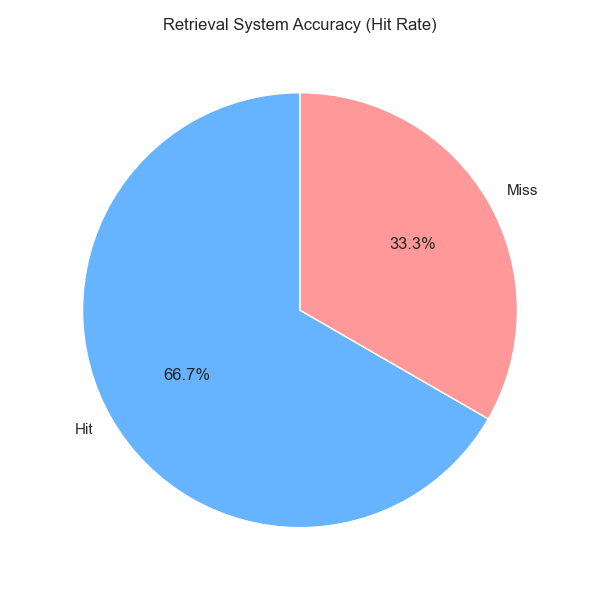
\includegraphics[width=0.6\textwidth]{retrieval_hit_rate.png}
    \caption{Retrieval System Accuracy showing the proportion of successful hits.}
    \label{fig:hit_rate}
\end{figure}

\subsubsection{Prompting Strategy Comparison}
We compared the three prompting strategies on a comprehensive dataset.

\begin{table}[H]
    \centering
    \caption{Performance Comparison of Prompting Strategies}
    \label{tab:performance}
    \begin{tabular}{lcc}
        \toprule
        \textbf{Strategy} & \textbf{Avg Latency (s)} & \textbf{ROUGE-L Score} \\
        \midrule
        Zero-shot & 2.86 & 0.11 \\
        Few-shot & 3.23 & \textbf{0.13} \\
        Chain-of-Thought & 5.43 & 0.07 \\
        \bottomrule
    \end{tabular}
\end{table}

\begin{figure}[H]
    \centering
    \begin{subfigure}{0.48\textwidth}
        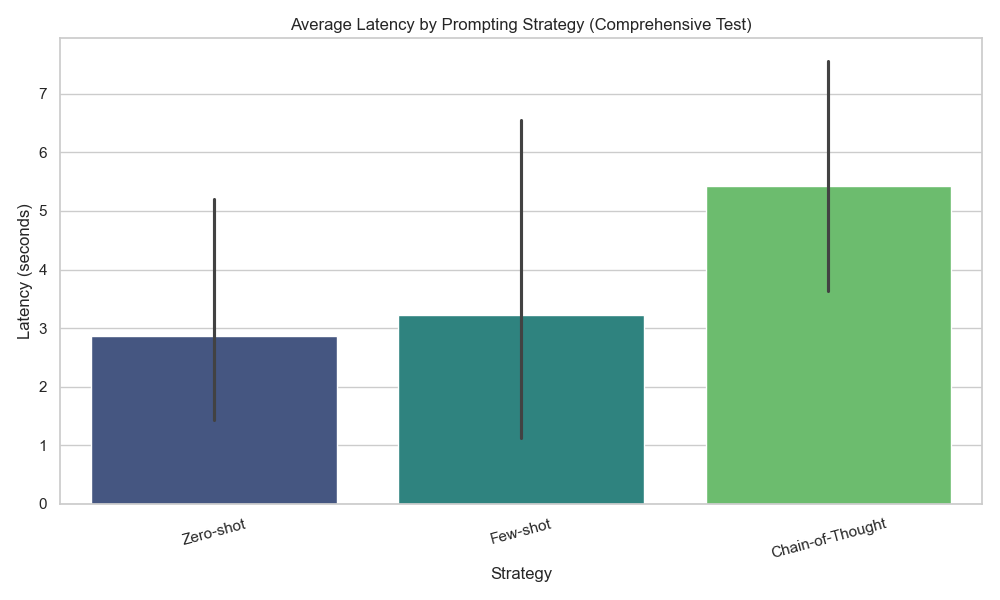
\includegraphics[width=\linewidth]{latency_comparison_comprehensive.png}
        \caption{Latency Comparison}
    \end{subfigure}
    \hfill
    \begin{subfigure}{0.48\textwidth}
        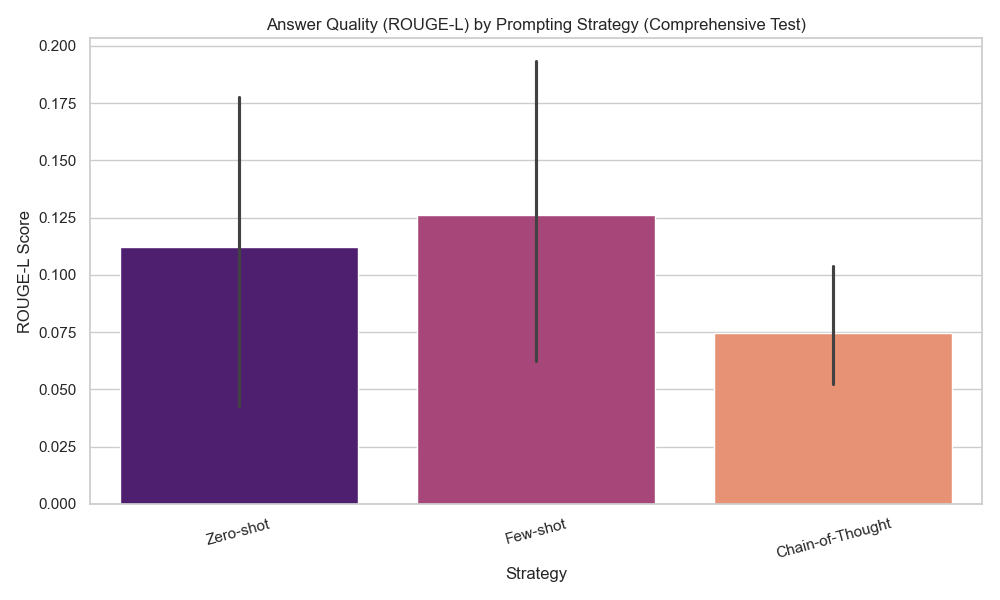
\includegraphics[width=\linewidth]{rouge_comparison_comprehensive.png}
        \caption{ROUGE Score Comparison}
    \end{subfigure}
    \caption{Impact of Prompting Strategies on Speed and Quality.}
    \label{fig:strategies}
\end{figure}

\textbf{Analysis}:
\begin{itemize}
    \item \textbf{Few-shot} achieved the highest quality (ROUGE-L: 0.13), proving that examples help the model adhere to the desired answer format.
    \item \textbf{Zero-shot} was the fastest (2.86s), making it ideal for real-time use.
    \item \textbf{Chain-of-Thought} incurred a significant latency penalty (5.43s) and scored lower on ROUGE, likely because its verbose reasoning steps did not match the concise ground truth references.
\end{itemize}

\subsection{Embedding Space Visualization}
To understand the vector space, we projected the 512-dimensional embeddings into 2D using PCA and t-SNE.

\begin{figure}[H]
    \centering
    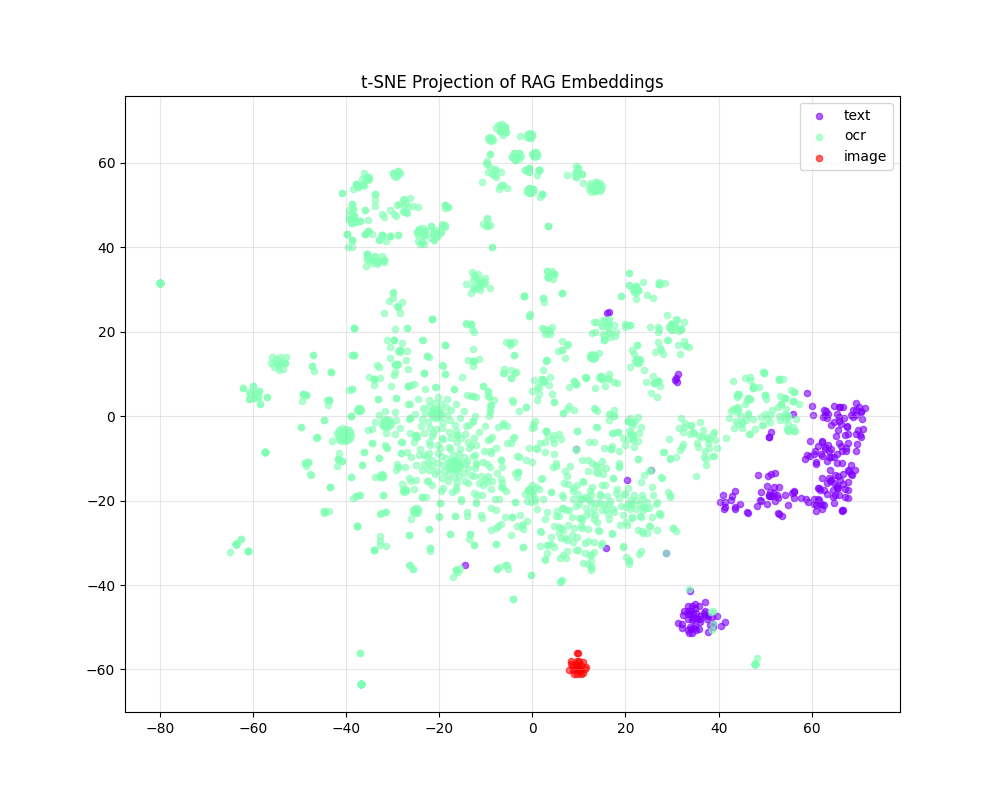
\includegraphics[width=0.8\textwidth]{embeddings_tsne.png}
    \caption{t-SNE Projection of Embeddings. Clusters indicate semantic similarity between text chunks and images.}
    \label{fig:tsne}
\end{figure}

The visualization reveals distinct clusters, confirming that the CLIP model successfully groups semantically related content (e.g., specific campus details or financial tables) together.

\section{Challenges and Solutions}

\begin{enumerate}
    \item \textbf{Challenge: Multimodal Alignment} \\
    \textit{Issue}: Text and images are inherently different modalities. \\
    \textit{Solution}: We used CLIP, which is explicitly trained to align these modalities in a shared vector space, enabling seamless cross-modal retrieval.

    \item \textbf{Challenge: Hallucinations} \\
    \textit{Issue}: The LLM would sometimes invent answers for queries not in the context. \\
    \textit{Solution}: We implemented a strict system prompt ("Use ONLY the provided context") and added negative tests (e.g., "recipe for cake") to verify the model correctly refuses to answer irrelevant questions.

    \item \textbf{Challenge: Windows Encoding Errors} \\
    \textit{Issue}: Python scripts failed due to emoji characters in print statements on Windows. \\
    \textit{Solution}: We sanitized the code to remove non-standard characters, ensuring cross-platform compatibility.
\end{enumerate}

\section{User Interface Implementation}
The system features a user-friendly interface built with Streamlit, allowing users to select prompting strategies and interact with the system via text or image queries.

\begin{figure}[H]
    \centering
    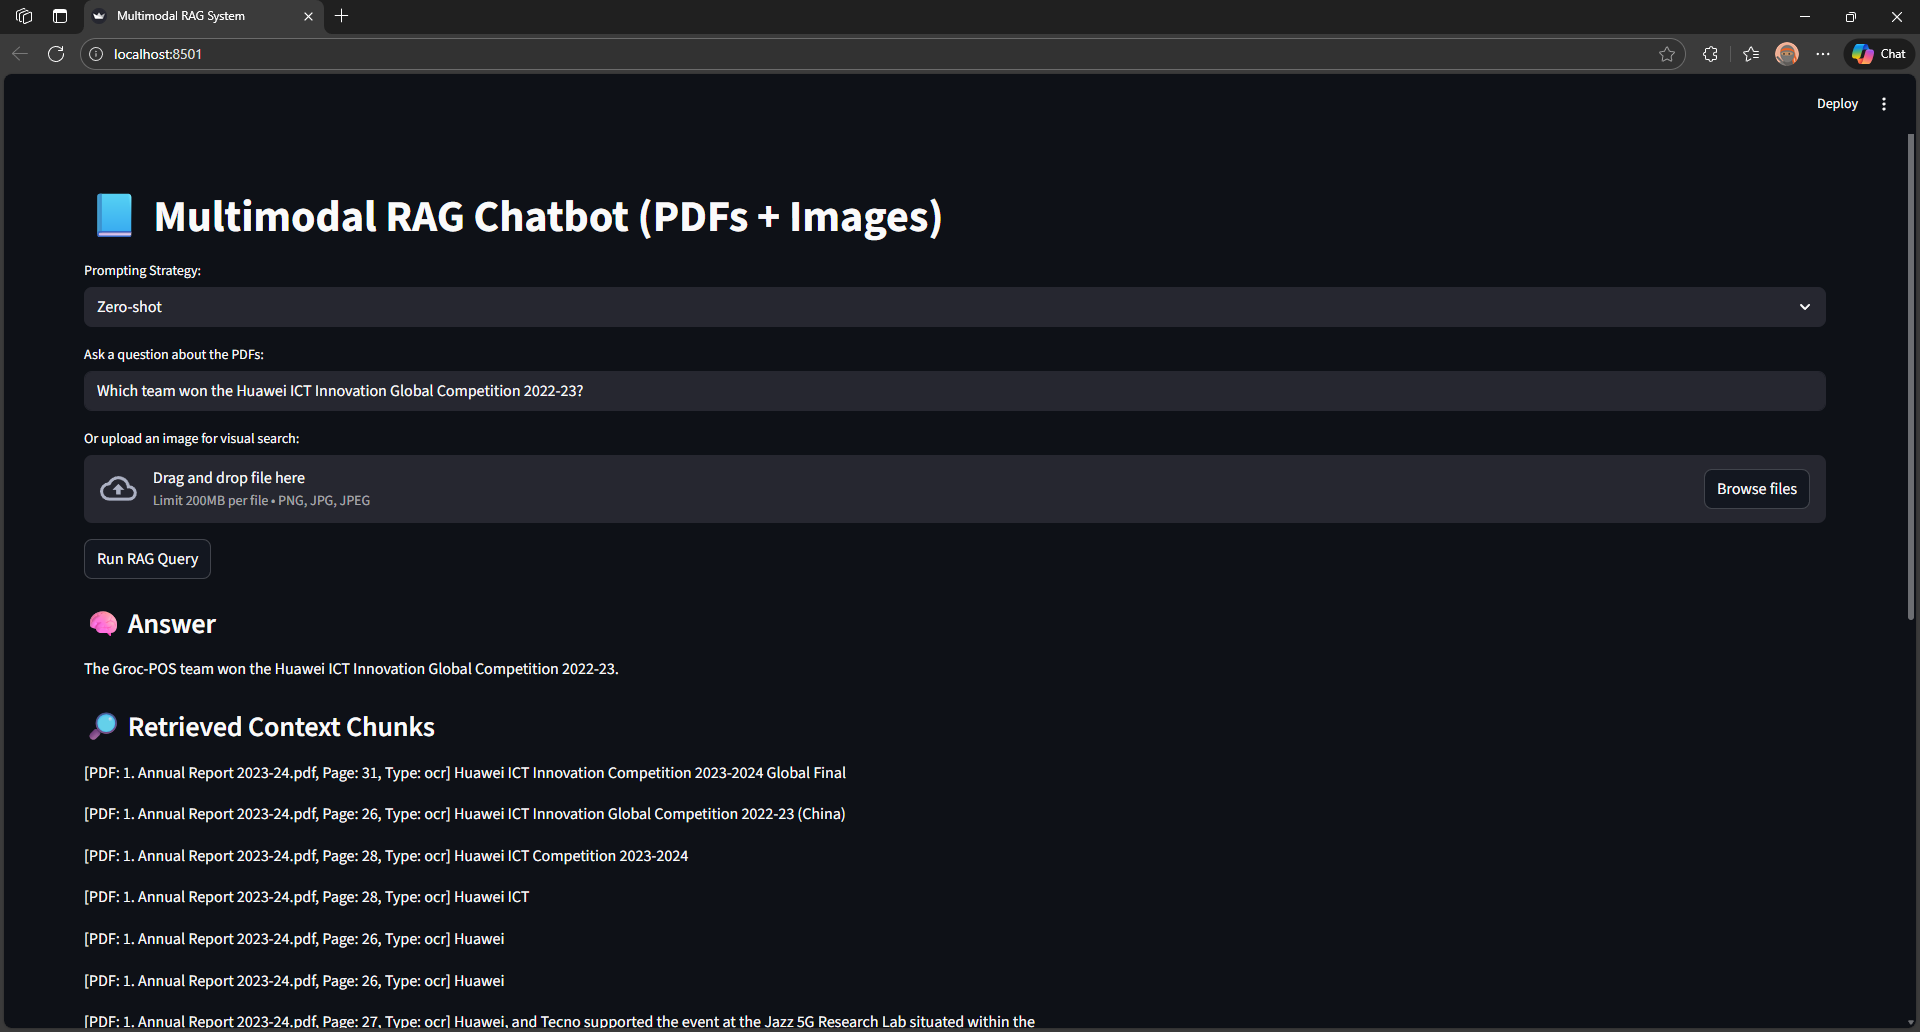
\includegraphics[width=0.9\textwidth]{Zero-shot.png}
    \caption{Zero-shot Prompting Interface: Direct question answering.}
    \label{fig:ui_zero}
\end{figure}

\begin{figure}[H]
    \centering
    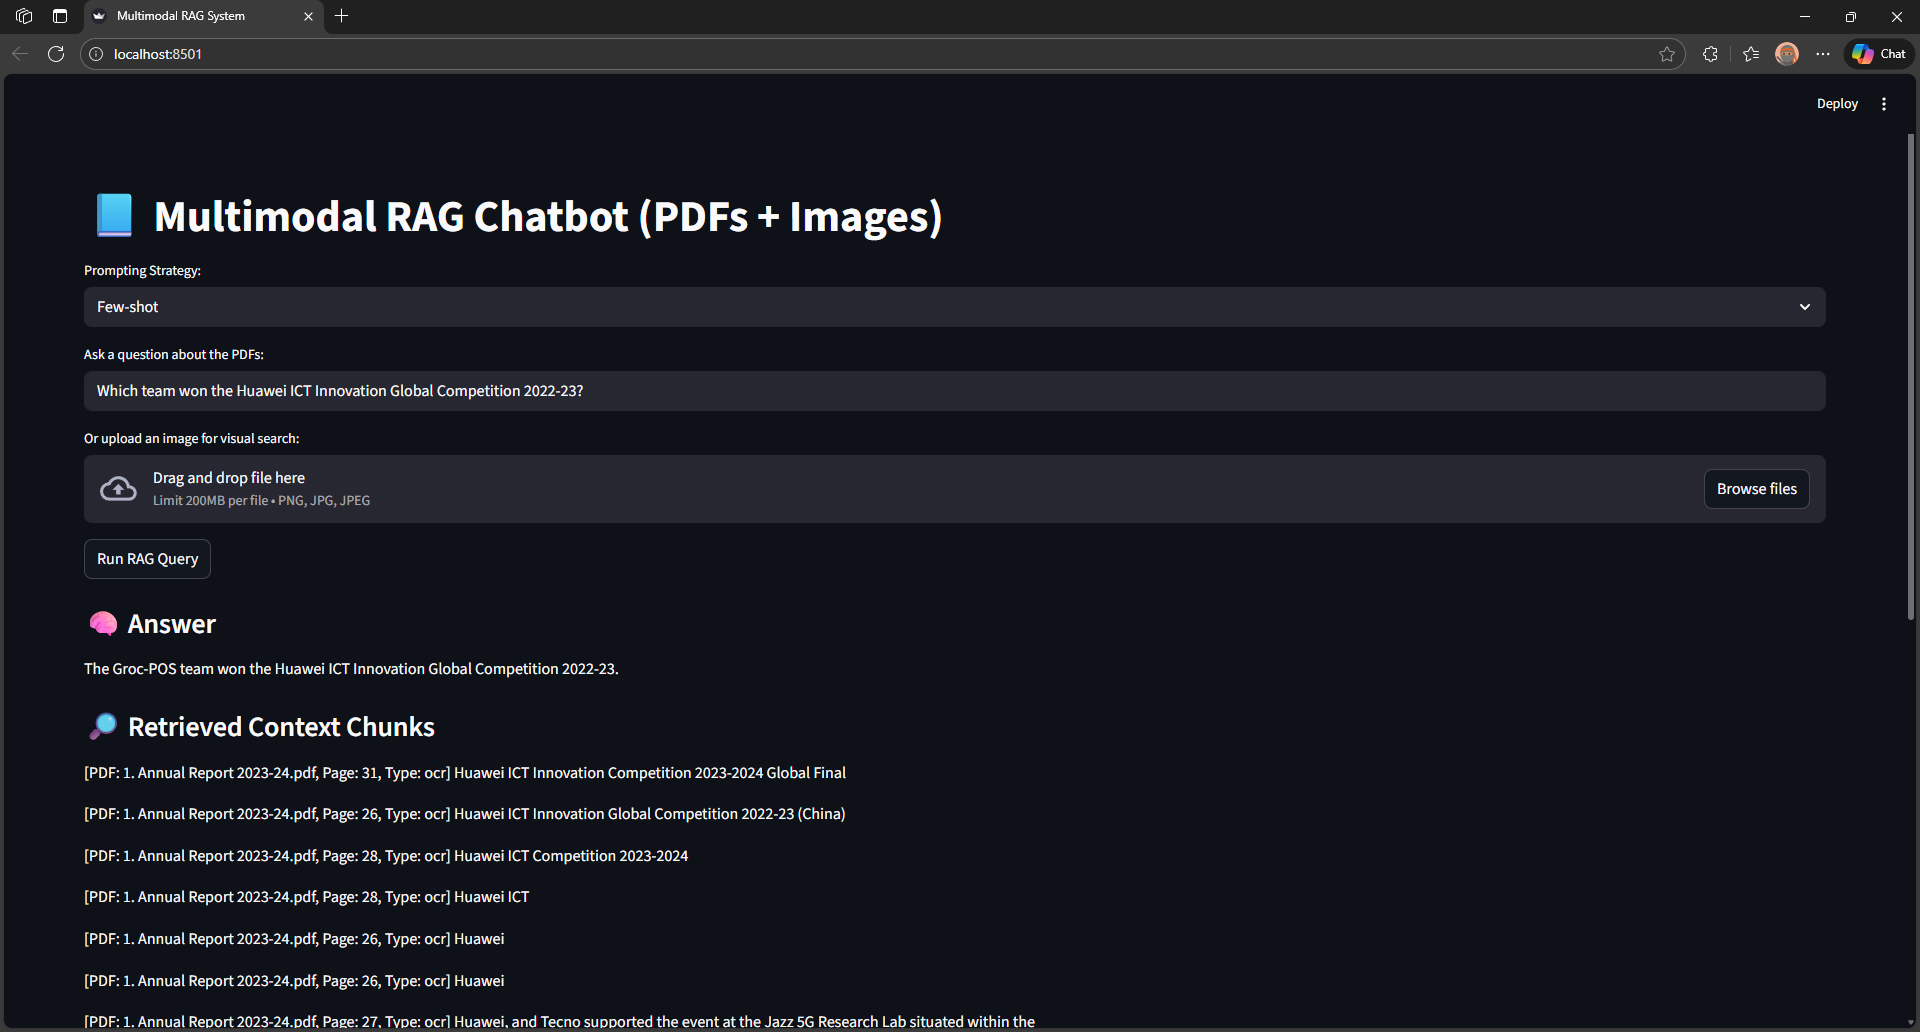
\includegraphics[width=0.9\textwidth]{Few-shot.png}
    \caption{Few-shot Prompting Interface: The model uses internal examples to guide the response style.}
    \label{fig:ui_few}
\end{figure}

\begin{figure}[H]
    \centering
    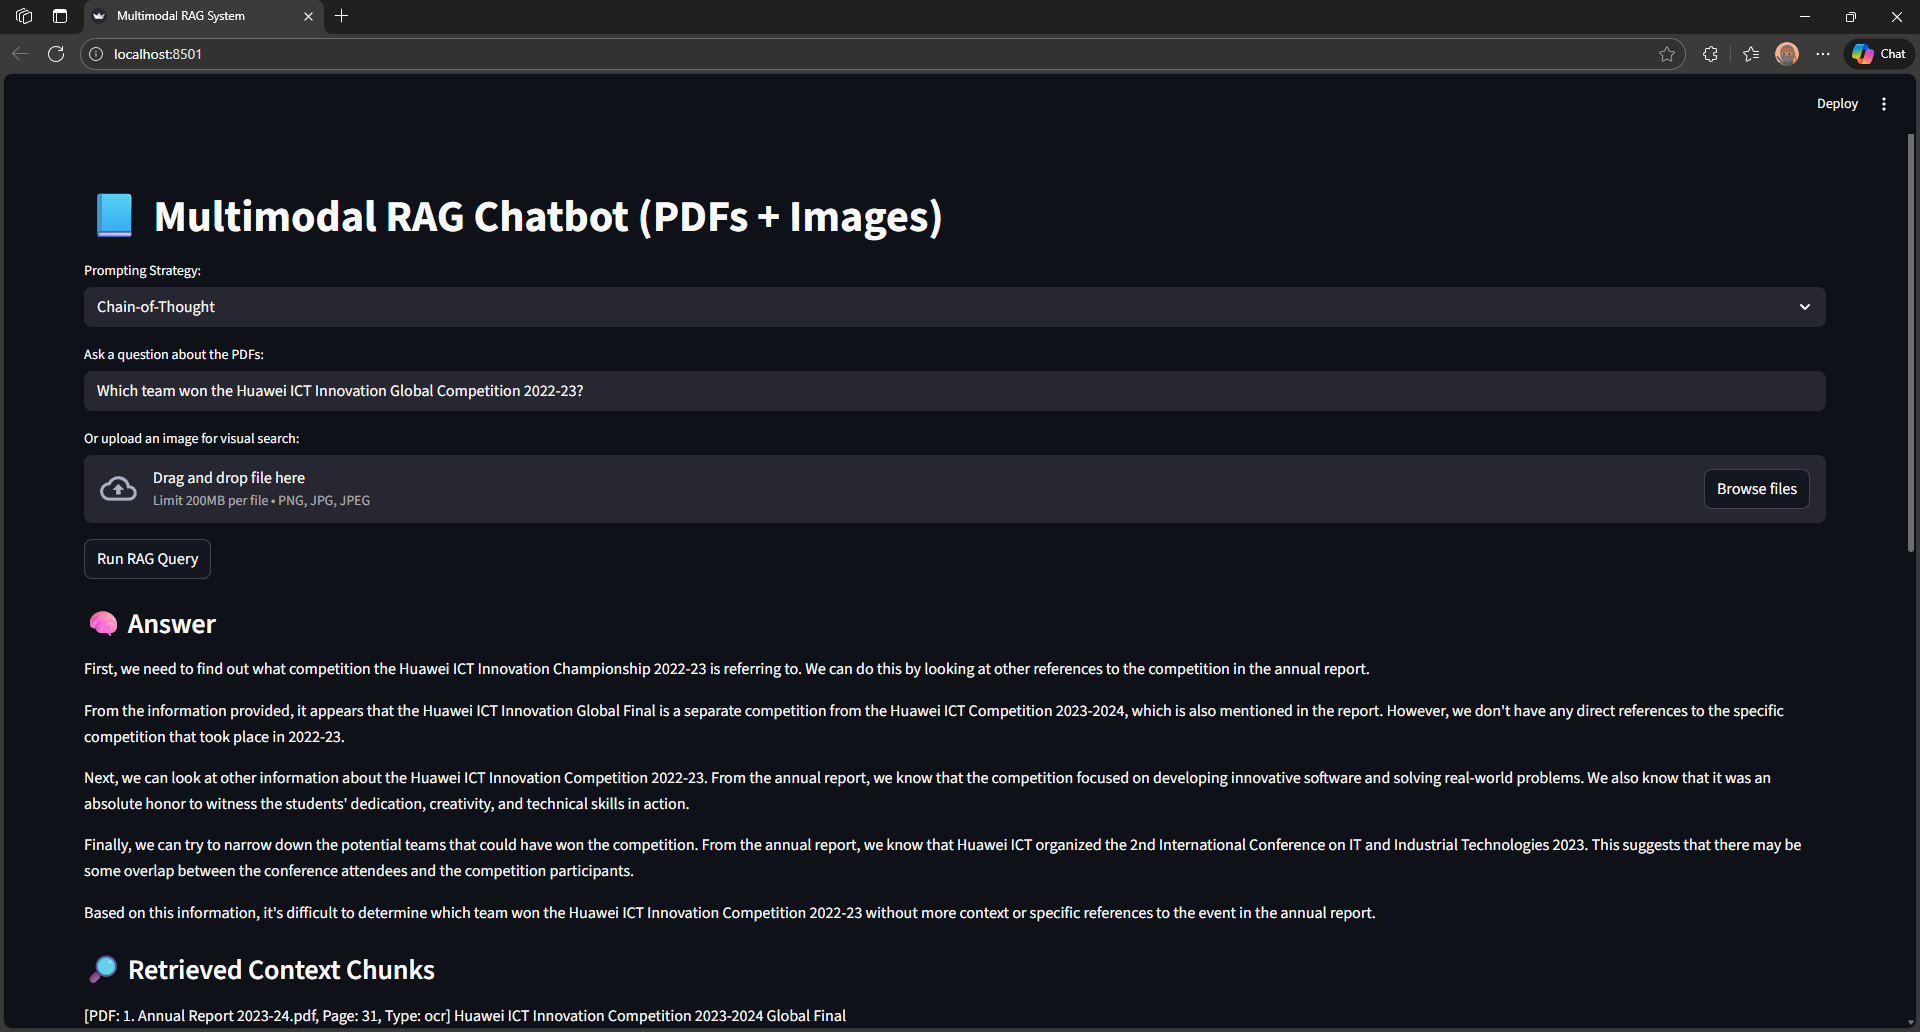
\includegraphics[width=0.9\textwidth]{COT.png}
    \caption{Chain-of-Thought Interface: The model displays step-by-step reasoning before the final answer.}
    \label{fig:ui_cot}
\end{figure}

\section{Conclusion}
We successfully developed a Multimodal RAG system that integrates PDF parsing, OCR, vector search, and local LLM generation. The evaluation demonstrates that \textbf{Few-shot prompting} offers the best balance of quality and performance. The system's ability to handle both text and image queries makes it a powerful tool for navigating complex documents like annual reports.

\end{document}
